\chapter{Viabilidad económica y proyección comercial}
\label{ch:viabilidad_economica}

Este capítulo analiza la viabilidad económica de Parky en un escenario de despliegue profesional real y que haría falta para convertir el prototipo actual en un producto comercializable. Se detallan las brechas entre el prototipo y una versión lista para el mercado, se presenta un plan de desarrollo con su coste asociado, y se analiza el modelo de ingresos proyectado junto con la estimación del retorno de la inversión a medio plazo.

% ============================================================
\section{Del prototipo al producto comercial}
\label{sec:prototipo_a_comercial}

El prototipo que este TFG documenta es ahora mismo totalmente funcional ya que un usuario puede registrarse, publicar una plaza, hacer una reserva, pagar con el motor de precios activo y abrir el acceso al garaje mediante SmartAccess. Eso cubre el flujo básico completo de extremo a extremo. Lo que no cubre es todo lo que un producto necesita antes de que alguien ponga dinero real en él.

La diferencia más importante es el procesamiento de pagos. El prototipo implementa la arquitectura de \textit{Stripe Connect} (los datos de la transacción, el desglose de comisión e IGIC, el modelo de pagos en base de datos) pero no ejecuta llamadas reales a la API de Stripe. El porque de esto no es un descuido sino que \textit{Stripe Connect} exige que la cuenta del propietario del \textit{marketplace} esté verificada como empresa y que cada vendedor complete un proceso de \textit{onboarding} con documentación de identidad. En Canarias, ese proceso implica acreditación fiscal ante la AEAT y alta en el Registro Mercantil, condiciones que están fuera del alcance de un proyecto académico y es por ello que se ha obviado toda esta parte. Para la versión comercial, la integración completa de Stripe Connect es el primer requisito no técnico que bloquea el lanzamiento y que se debe implementar para generar ingresos.

El segundo bloque de trabajo pendiente es la presencia en tiendas de aplicaciones. El APK de Android funciona y se ha validado en dispositivos reales, pero publicarlo en Google Play exige superar una revisión de contenido y tener una cuenta de desarrollador activa. La versión iOS no existe porque Capacitor requiere un Mac con Xcode para compilarla, y la revisión de App Store de Apple añade una capa de aprobación adicional con tiempos de respuesta de varios días a parte de tener obligatoriamente una cuenta de desarrollador la cual necesita un desembolso de 100 euros para poder publicar en el App Store. Para el lanzamiento en Canarias, que combina usuarios web con usuarios móviles, ambas plataformas son necesarias y fundamentales ya que la versión comercial se basa fundamentalmente en la presencia en dispositivos móviles.

Quedan también obligaciones legales. La plataforma intermedia entre propietarios y conductores, lo que la sitúa en un escenario de responsabilidad civil ante conflictos como pueden ser los daños en la plaza, disputas de facturación, cobros incorrectos y un largo etc. Una versión comercial necesita condiciones generales de uso redactadas por un jurista, una política de privacidad conforme al RGPD y al procedimiento de ejercicio de derechos ARCO, y un mecanismo de resolución de disputas. Nada de esto existe en el prototipo pero si es obligatorio para el lanzamiento comercial.

Finalmente, operar con usuarios reales requiere monitorización. Vercel y Supabase incluyen métricas básicas, pero un producto en producción necesita alertas sobre errores en tiempo real, análisis de rendimiento por endpoint y un canal de soporte accesible.

% ============================================================
\section{Funcionalidades de la versión avanzada}
\label{sec:funcionalidades_adicionales}

Más allá de completar los requisitos del lanzamiento, una versión avanzada de Parky añadiría funcionalidades adicionales que mejorarían exponencialmente la experiencia del usuario medio haciendola más atractiva a su público objetivo.

\paragraph{Detección pasiva de estacionamiento.}
Capacitor puede monitorizar en segundo plano la conexión Bluetooth con el manos libres del vehículo ya que prácticamente todos los vehículos modernos lo soportan. Con esta funcionalidad, al apagar el motor, el dispositivo registra la geolocalización y puede compararla con la de la plaza para confirmar la ocupación sin que el usuario tenga que abrir la aplicación, y de igual modo, al arrancar, la marca automáticamente como libre, sin que el usuario tenga que abrir la aplicación de cara a terminar la reserva pudiendo maximizar el tiempo de uso de la plaza con más usuarios.

\paragraph{Pases temporales y abonos recurrentes.}
Con \textit{Stripe Billing} se podrían añadir dos modalidades de reserva recurrente: un \textit{EventPass} que agrupa plazas cercanas a un recinto a tarifa fija durante eventos masivos (el Estadio Heliodoro Rodríguez López o el Recinto Ferial de Tenerife, por ejemplo) y un \textit{SeasonPass} para conductores habituales que repiten el mismo trayecto en franjas fijas, como el personal de la Universidad de La Laguna. De este modo, se amplía el espectro de clientes potenciales y se fideliza a usuarios recurrentes con necesidades de aparcamiento predecibles.

\paragraph{Validación automática ante la ZBE.}
Al confirmar una reserva dentro de la ZBE de Santa Cruz de Tenerife, un \textit{webhook} de Supabase consulta la plataforma municipal y recibiría un JWT firmado que exime al conductor de sanción administrativa haciendo el proceso transparente para el usuario. Esto no solo mejora la experiencia del usuario sino que también posiciona a Parky como un facilitador de movilidad sostenible, alineándose con las políticas de reducción de emisiones en zonas urbanas y aumentando su atractivo para conductores de vehículos eléctricos e híbridos.

\paragraph{Tarificación de recarga para vehículos eléctricos.}
Para plazas con cargador doméstico, el motor de precios incorpora el coste eléctrico del PVPC\footnote{\textbf{PVPC} (\textit{Precio Voluntario para el Pequeño Consumidor}): Tarifa regulada de electricidad en España cuyo precio varía por hora según el mercado mayorista.} en tiempo real. Stripe Connect separa el coste energético del aparcamiento al liquidar el servicio. Con esto, el arrendatario paga una tarifa base por hora de aparcamiento más el coste variable de la recarga en una sola transacción, mientras que el arrendador recibe ambos conceptos por separado, lo que incentiva la oferta de plazas con puntos de recarga y posiciona a Parky como una plataforma comprometida con la movilidad eléctrica.

\paragraph{Precios dinámicos por demanda contextual.}
El motor actual de \texttt{pricing.service.ts} usa multiplicadores estáticos por día y tramo horario. Esta funcionalidad añadiría tres señales adicionales: eventos próximos detectados vía APIs de agenda cultural y deportiva de Tenerife, ocupación histórica por franja horaria en la zona, y días de inactividad de la plaza. El precio sube cuando hay demanda real y baja cuando la plaza lleva tiempo vacía haciendo el sistema más inteligente y adaptativo a las condiciones del mercado, lo que maximiza los ingresos para los propietarios y mejora la disponibilidad para los conductores.

\paragraph{Programa de reputación y verificación de usuarios.}
Inspirado en plataformas como Airbnb y Uber, un sistema de puntuación bidireccional donde tanto propietarios como conductores califican mutuamente tras cada transacción(actualmente está el sistema de review instaurado para los dueños de plazas). Los usuarios con reputación consistentemente alta (4,5 puntos o más) acceden a tarifas especiales reducidas en un 5\,\% y a plazas exclusivas. Adicionalmente, la verificación mediante documento de identidad, datos bancarios y antecedentes de conducción genera un distintivo de \textit{usuario verificado} que incrementa la confianza en la plataforma y reduce fraudes, siendo especialmente relevante para propietarios de plazas en zonas premium.

\paragraph{Sistema de reservas recurrentes automáticas y cancelación flexible.}
Siguiendo el modelo de aplicaciones como Spotify o Netflix, los usuarios pueden configurar suscripciones de aparcamiento que se auto-renuevan en franjas fijas (por la mañana antes de trabajar, para citas al médico recurrentes, etc.). Ofrece descuentos escalonados: 5\,\% por cinco reservas mensuales confirmadas, 10\,\% por diez. Incluye una política de cancelación flexible sin penalización si se avisa con al menos 24 horas de anticipación, mejorando la experiencia del usuario habitual y generando ingresos predecibles sin comprometer la fluidez de la plataforma.

\paragraph{Integración de mapas interactivos con información en tiempo real.}
Amplía Leaflet con capas adicionales como son ocupación actual de plazas en tonos de color (verde disponible, rojo ocupado), superposición de zonas de restricción de tráfico (ZBE, horarios de carga-descarga), estaciones de recarga eléctrica cercanas y puntos de interés (comercios, hospitales, estaciones de transporte). Similar a lo que ofrece Google Maps y Apple Maps, la visualización integrada reduce fricción en la búsqueda y proporciona contexto inmediato para la toma de decisiones del usuario, mejorando significativamente la experiencia de descubrimiento de plazas.

\paragraph{Dibujar en el mapa el area de búsqueda personalizada.}
En lugar de limitar la búsqueda a un radio fijo, el usuario puede dibujar un polígono personalizado en el mapa para definir su área de interés. Esto es especialmente útil y ya lo implementan aplicaciones como Idealista y otras plataformas de compra-venta. La plataforma ajusta dinámicamente los resultados de búsqueda y las recomendaciones de plazas dentro del área definida, ofreciendo una experiencia de búsqueda más flexible y adaptada a las necesidades reales del usuario.

% ============================================================
\section{Planificación y coste de la versión comercial}
\label{sec:desarrollo_proyecto}

La planificación sigue un ciclo de vida en cinco fases, con la fase de pruebas ejecutada en paralelo al desarrollo a partir del quinto mes. El equipo se contrata mediante subcontratación a una consultora de software, de modo que la tarifa horaria ya consolida los costes de seguridad social, equipamiento y margen de intermediación. La figura~\ref{fig:gantt} muestra el diagrama exportado desde ProjectLibre.

\paragraph{Análisis (35 días).}
Recogida de requisitos funcionales y no funcionales, modelado de la lógica de reservas y tarifas, revisión de la normativa de \textit{ZBE} aplicable en Tenerife y validación del tratamiento fiscal del IGIC sobre las comisiones de la plataforma. Participan el Jefe de Proyecto, el Analista y el Arquitecto de Software.

\paragraph{Diseño (30 días).}
Definición de la arquitectura del sistema: esquema de base de datos PostgreSQL con políticas RLS, elección del ecosistema tecnológico (React~18, TypeScript, Supabase, Capacitor) y elaboración de prototipos de interfaz para web y Android con validación temprana de usabilidad.

\paragraph{Desarrollo (142 días).}
La fase central ejecuta cuatro frentes en paralelo: el \textit{backend} con Supabase y Edge Functions (80 días), el \textit{frontend} web en React~18 (85 días, camino crítico), la aplicación Android con Capacitor (61 días) y el módulo SmartAccess para apertura remota de garajes mediante código QR y registro de eventos de acceso (35 días). La integración completa de Stripe Connect, que gestiona el reparto automático de comisiones entre arrendador y plataforma, se ejecuta dentro del bloque de \textit{backend}.

\paragraph{Pruebas (91 días).}
Fase paralela al desarrollo desde el quinto mes. Cubre pruebas unitarias, de integración entre servicios, de rendimiento bajo carga concurrente, de usabilidad con usuarios reales y pruebas de aceptación previas al despliegue.

\paragraph{Despliegue (12 días).}
Configuración de entornos de producción en Vercel para el \textit{frontend} y Supabase para el \textit{backend}, publicación de la aplicación en Google Play y App Store, y auditoría de seguridad previa al lanzamiento público.

\begin{figure}[htbp]
    \centering
    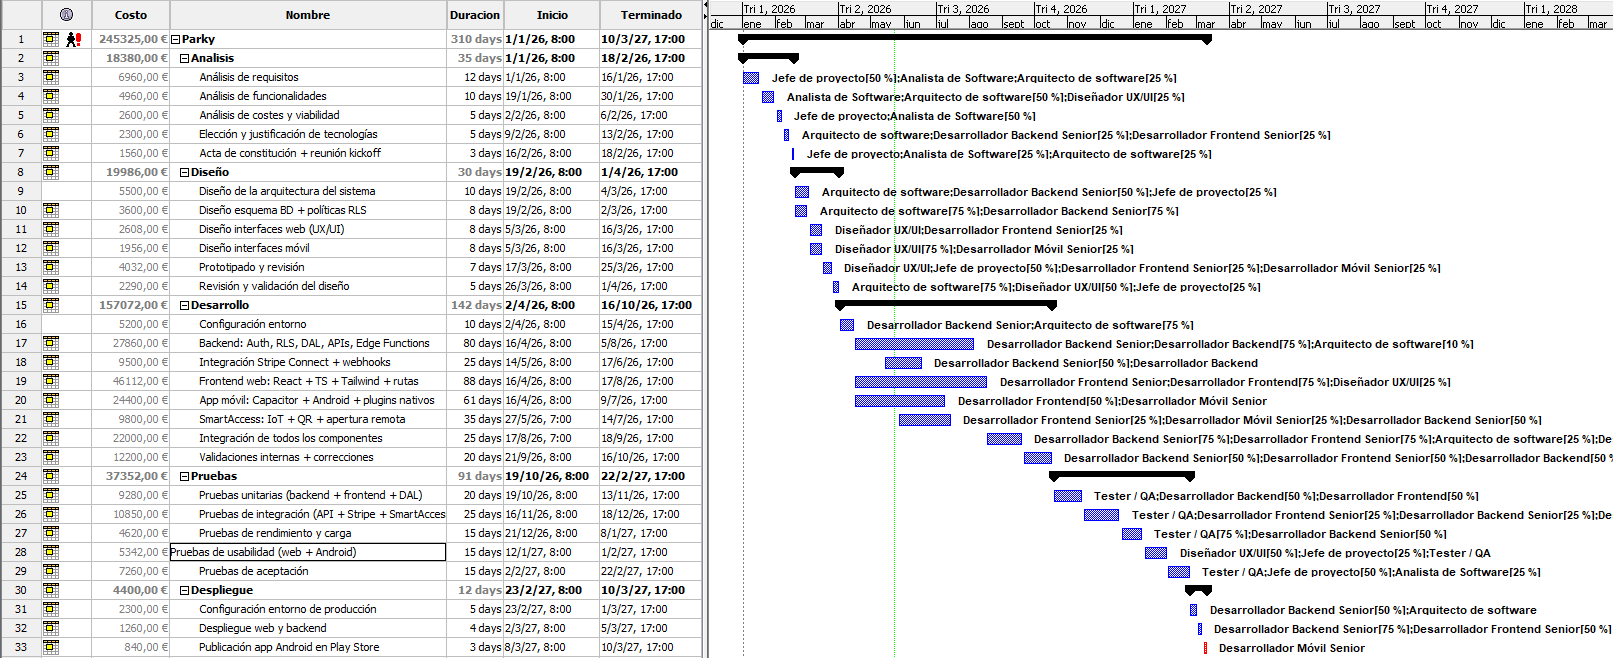
\includegraphics[width=\textwidth]{images/assets/GANTT/GANTT}
    \vspace{2pt}
    \caption{Diagrama de Gantt del proyecto Parky exportado desde ProjectLibre~\cite{projectlibre2026parky} (enero 2026 -- marzo 2027). La franja superior cubre enero--junio 2026; la inferior, julio 2026--marzo 2027.}
    \label{fig:gantt}
\end{figure}

\subsection{Equipo y coste del proyecto}
\label{subsec:coste_duracion}

El equipo mínimo necesario cubre diez perfiles técnicos. Al subcontratar a una consultora, la tarifa horaria absorbe los costes de seguridad social, licencias de software internas y equipamiento de la agencia. El proyecto requiere además hardware específico para validar la experiencia nativa en dispositivos móviles.

\begin{table}[htbp]
    \centering
    \renewcommand{\arraystretch}{1.2}
    \begin{tabular}{lccc}
        \toprule
        \textbf{Perfil técnico}                                                                                                                                        & \textbf{Horas est.} & \textbf{Tarifa (€/h)} & \textbf{Coste (€)}  \\
        \midrule
        Jefe de Proyecto                                                                                                                                               & 300,00              & 45                    & 13.500,00           \\
        Analista de Software                                                                                                                                           & 224,00              & 40                    & 8.960,00            \\
        Arquitecto de Software                                                                                                                                         & 478,00              & 40                    & 19.120,00           \\
        Diseñador UI/UX                                                                                                                                                & 444,00              & 32                    & 14.208,00           \\
        Desarrollador Frontend Senior                                                                                                                                  & 1.106,00            & 35                    & 38.710,00           \\
        Desarrollador Frontend                                                                                                                                         & 1.032,00            & 30                    & 30.960,00           \\
        Desarrollador Móvil Senior                                                                                                                                     & 758,00              & 35                    & 26.530,00           \\
        Desarrollador Backend Senior                                                                                                                                   & 1.242,00            & 35                    & 43.470,00           \\
        Desarrollador Backend                                                                                                                                          & 790,00              & 30                    & 23.700,00           \\
        Tester / QA\footnote{\textbf{QA} (\textit{Quality Assurance}): perfil responsable de validar la calidad del software antes de su liberación al usuario final.} & 644,00              & 28                    & 18.032,00           \\
        \midrule
        \textbf{Subtotal personal}                                                                                                                                     & \textbf{7.018,00}   & ---                   & \textbf{237.190,00} \\
        \bottomrule
    \end{tabular}
    \caption{Presupuesto por perfil técnico.}
    \label{tab:presupuesto_equipo}
\end{table}

\begin{table}[htbp]
    \centering
    \renewcommand{\arraystretch}{1.2}
    \begin{tabular}{lcc}
        \toprule
        \textbf{Concepto}                    & \textbf{Uds.} & \textbf{Coste (€)}  \\
        \midrule
        Portátil de desarrollo               & 4             & 4.800,00            \\
        Smartphone iOS (pruebas nativas)     & 2             & 1.800,00            \\
        Smartphone Android (pruebas nativas) & 2             & 1.200,00            \\
        Licencias IDE (JetBrains)            & 1             & 320,00              \\
        Dominio web y registro DNS           & 1             & 15,00               \\
        \midrule
        Subtotal material                    &               & 8.135,00            \\
        Subtotal personal                    &               & 237.190,00          \\
        \midrule
        \textbf{Coste total del proyecto}    &               & \textbf{245.325,00} \\
        \bottomrule
    \end{tabular}
    \caption{Recursos materiales y coste total del proyecto.}
    \label{tab:recursos_material}
\end{table}

Estos costes cubren el desarrollo. Para absorber imprevistos técnicos, los gastos operativos durante el período de rodaje y la campaña publicitaria de lanzamiento en las Islas Canarias, se recomienda una inversión de capital no inferior a 350.000 euros.

% ============================================================
\section{Modelo de comercialización}
\label{sec:modelo_comercializacion}

Parky opera como un \textit{marketplace} bilateral en el que la plataforma actúa como intermediaria sin poseer el inventario físico. La monetización se articula en tres vías independientes que cubren desde la transacción puntual hasta el cliente recurrente de alto volumen.

\subsection{Comisión transaccional bilateral}
\label{subsec:comision_transaccional}

Por cada reserva completada, la plataforma aplica una estructura asimétrica: el arrendador cede un 3\,\% del precio base ($\beta = 0{,}03$), cuota que absorbe el coste de procesamiento bancario de Stripe Connect; el arrendatario abona una comisión de servicio del 12\,\% ($\alpha = 0{,}12$) más una tasa fija de gestión de 0,50\,€ ($F_t$). El precio final desembolsado por el arrendatario es:
\[
    P_d = P_b \cdot (1 + \alpha) + F_t
\]
donde $P_b$ es el precio base fijado por el propietario. El ingreso total retenido por la plataforma por transacción agrega ambos flujos:
\[
    I_{\text{plataforma}} = P_b \cdot (\alpha + \beta) + F_t
\]
El 3\,\% que aporta el arrendador cubre el cargo de Stripe (1,4\,\%--2,9\,\% + 0,30\,€), de modo que el margen neto de la plataforma recae principalmente sobre la comisión del arrendatario. Las Edge Functions de Supabase calculan automáticamente el IGIC del 7\,\% sobre las comisiones de servicio y Stripe Connect transfiere el saldo neto al arrendador sin intervención manual.

\subsection{Parky Pro: suscripción para multipropietarios}
\label{subsec:parky_pro}

Gestores inmobiliarios, administradores de fincas y propietarios con carteras de más de tres plazas pueden contratar una suscripción mensual vía Stripe Billing que elimina la comisión del arrendador ($\beta = 0$) a cambio de una cuota fija recurrente. El plan Basic Pro (19\,€/mes) da acceso a paneles de analítica en tiempo real sobre Supabase, actualización masiva de tarifas e integración con el calendario de eventos de Tenerife. El plan Advanced Pro (39\,€/mes) añade la exención completa de la comisión de arrendador, gestión de hasta 20 plazas y soporte para la declaración trimestral del IGIC. Ambos niveles garantizan ingresos predecibles para la plataforma incluso en períodos de baja demanda transaccional.

\subsection{Visibilidad premium}
\label{subsec:visibilidad_premium}

Los propietarios pueden adquirir mejoras de posicionamiento de pago único mediante cobro in-app. Un \textit{Destacado de Zona} (1,99\,€ por 3 días) eleva algorítmicamente la plaza en los listados de búsqueda cercanos y diferencia el marcador en el mapa de Leaflet mediante un color exclusivo. Un \textit{Posicionamiento Urgente} (4,99\,€ por 7 días) muestra la plaza con prioridad a conductores que se aproximan a la zona durante eventos de alta demanda, como partidos en el Estadio Heliodoro Rodríguez López o congresos en la Universidad de La Laguna. Ambas modalidades generan ingresos directos sin incrementar la comisión base ni penalizar a los usuarios no suscritos.

% ============================================================
\section{Estimación del retorno de la inversión}
\label{sec:estimacion_roi}

El retorno de la inversión (ROI\footnote{\textbf{ROI} (\textit{Return on Investment}): cociente entre el beneficio neto obtenido y la inversión inicial, expresado habitualmente como porcentaje.}) confronta los gastos acumulados con los ingresos generados por las tres vías de monetización descritas en la sección anterior. La proyección toma un escenario conservador: penetración gradual en el área metropolitana de Tenerife, sin viralización anómala ni campañas de gran alcance durante los primeros meses de operación.

La inversión inicial de 350.000 euros se reparte entre el coste de desarrollo (245.325,00 euros) y un fondo operativo de 104.675,00 euros destinado a publicidad en redes sociales y plataformas de agregadores durante los primeros seis meses, más los gastos corrientes de infraestructura (Supabase, Vercel y herramientas de monitorización, estimados en unos 2.000 euros mensuales) hasta que la curva de ingresos alcance flujo de caja positivo.

Las hipótesis de partida son las siguientes: el mercado objetivo comprende aproximadamente 45.000 conductores urbanos activos en el área de Santa Cruz de Tenerife y La Laguna; se estima que entre el 2\,\% y el 3\,\% de los usuarios registrados completa reservas de pago de forma recurrente semanal, porcentaje habitual en plataformas P2P con fricción de confianza moderada~\cite{grandviewresearch2022}; el precio medio de reserva se sitúa en 9,00\,€ (seis horas a 1,50\,€/h), generando un ingreso neto por transacción de aproximadamente 2,35\,€ una vez descontado el IGIC. A partir del cuarto mes se añaden ingresos recurrentes por suscripciones Parky Pro y, desde el tercer mes, micropagos por visibilidad premium, lo que acelera la curva de ingresos respecto a un modelo puramente transaccional.

\begin{table}[htbp]
    \centering
    \renewcommand{\arraystretch}{1.2}
    \begin{tabular}{cccc}
        \toprule
        \textbf{Mes comercial}                & \textbf{Gastos acumulados (€)} & \textbf{Ingresos acumulados (€)} & \textbf{Balance (€)} \\
        \midrule
        Mes 1                                 & 352.000                        & 1.200                            & $-$350.800           \\
        Mes 4                                 & 358.500                        & 20.000                           & $-$338.500           \\
        Mes 8                                 & 364.000                        & 85.000                           & $-$279.000           \\
        Mes 12                                & 369.000                        & 200.000                          & $-$169.000           \\
        Mes 15                                & 373.000                        & 305.000                          & $-$68.000            \\
        \textbf{Mes 18 (punto de equilibrio)} & \textbf{377.000}               & \textbf{385.000}                 & \textbf{+8.000}      \\
        Mes 21                                & 381.000                        & 530.000                          & +149.000             \\
        Mes 24                                & 385.000                        & 720.000                          & +335.000             \\
        \bottomrule
    \end{tabular}
    \caption{Evolución proyectada de gastos frente a ingresos y punto de equilibrio.}
    \label{tab:roi}
\end{table}

El punto de equilibrio se alcanza en el decimoctavo mes comercial, cuando los ingresos acumulados de las tres vías superan por primera vez los gastos totales. El mes 18 coincide con el período en que las suscripciones Parky Pro alcanzan una base de usuarios estable y los ingresos por visibilidad se vuelven predecibles, reduciendo la dependencia del volumen transaccional puro. En el mes 24, con dos años completos de operación, el balance neto favorable roza los 335.000 euros, lo que confirma la recuperación de la inversión a medio plazo bajo un escenario de crecimiento moderado en el mercado del aparcamiento privado en Tenerife.
